\chapter*{Esperimento 6: Lettura e plot di un'onda con ADC e DMA}
\addcontentsline{toc}{chapter}{Esperimento 6: Lettura e plot di un'onda con ADC e DMA}

\section*{Obiettivo}
Leggere un onda generata tramite un generatore di funzioni, trasmettere i valori a MATLAB e plottarli usando il DMA sia per l'ADC che per la seriale.

\section*{Svolgimento\footnote{Nella repository è il progetto Exp08}}
Tramite CubeMX impostiamo ADC1 e USART3 come nell'esperimento precedente.

Inoltre colleghiamo l'ADC al DMA e l'UART al DMA: in particolare avremo il DMA2 Stream 0 collegato all'ADC1 e il DMA1 Stream 3 collegato ad USART3.

Impostiamo TIM2 per generare un update a $1\si{MHz}$:
\begin{displaymath}
 1 \si{MHz} = \frac{84\si{MHz}}{(84)}
\end{displaymath}

Questa frequenza di campionamento è stata scelta in quanto il nostro ADC è limitato ad una frequenza massima di $1.4\si{MHz}$:
\begin{itemize}
    \item Il clock source dell'ADC è $84\si{MHz}$
    \item Il minimo valore di prescaler impostabile per l'ADC è 4, quindi il clock in ingresso all'ADC è $84 \si{MHz} / 4 = 21 \si{MHz}$
    \item L'ADC impiega 15 cicli di clock per effettuare una conversione quindi la frequenza massima è $21 \si{MHz} / 15 = 1.4 \si{MHz}$
\end{itemize}

Effettuiamo il setup di ADC e USART come visto nello scorso esperimento.
Inoltre abilitiamo il bit per abilitare le richieste DMA.

\begin{minted}
[
frame=lines,
framesep=2mm,
baselinestretch=1.2,
fontsize=\footnotesize,
]{C}
//Turn on DMA mode
ADC1->CR2 |= ADC_CR2_DMA;

//Turn on DMA on transmission
USART3->CR3 |= USART_CR3_DMAT;
\end{minted}

Andiamo poi a fare il setup dei due DMA
\begin{minted}
[
frame=lines,
framesep=2mm,
baselinestretch=1.2,
fontsize=\footnotesize,
]{C}
/* setup DMA2 stream 0 - ADC */
	//set number of elements
	DMA2_Stream0->NDTR = SIZE;
	//set source peripheral address
	DMA2_Stream0->PAR = (uint32_t) &ADC1->DR;
	//set destination memory address
	DMA2_Stream0->M0AR = (uint32_t) buffer;
	//set half word memory data size
	DMA2_Stream0->CR |= DMA_SxCR_MSIZE_0;
	//set half word peripheral size
	DMA2_Stream0->CR |= DMA_SxCR_PSIZE_0;
	//enable transfer complete interrupt
	DMA2_Stream0->CR |= DMA_SxCR_TCIE;
	
	
  /* Setup DMA1 UART */
	//Disable DMA
	DMA1_Stream3->CR &= ~DMA_SxCR_EN;
	//set number of elements (multiply by 2 because we send bytes)
	DMA1_Stream3->NDTR = SIZE*2;
	//set source memory address
	DMA1_Stream3->M0AR = (uint32_t) buffer;
	//set destination peripheral address
	DMA1_Stream3->PAR = (uint32_t) &USART3->DR;
	//set byte memory data size
	DMA1_Stream3->CR &= ~DMA_SxCR_MSIZE_0;
	DMA1_Stream3->CR &= ~DMA_SxCR_MSIZE_1;
	//set byte peripheral size
	DMA1_Stream3->CR &= ~DMA_SxCR_PSIZE_0;
	DMA1_Stream3->CR &= ~DMA_SxCR_PSIZE_1;
	//enable transfer complete interrupt
	DMA1_Stream3->CR |= DMA_SxCR_TCIE;
\end{minted}

Andiamo poi ad abilitare il DMA2 (quello collegato all'ADC) e il TIM2 per far partire le conversioni
\begin{minted}
[
frame=lines,
framesep=2mm,
baselinestretch=1.2,
fontsize=\footnotesize,
]{C}
//Enable DMA2 
DMA2_Stream0->CR |= DMA_SxCR_EN;
//Enable TTM2 (start ADC conversion)
TIM2->CR1 |= TIM_CR1_CEN;
\end{minted}

Quando il DMA2 avrà riempito tutto il buffer verrà sollevato un interrupt.
Nella routine di questo interrupt andiamo a disabilitare il TIM2 e accendiamo il DMA1 per far partire la trasmissione dei dati con la seriale.
\begin{minted}
[
frame=lines,
framesep=2mm,
baselinestretch=1.2,
fontsize=\footnotesize,
]{C}
void DMA2_Stream0_IRQHandler(void)
{
  /* USER CODE BEGIN DMA2_Stream0_IRQn 0 */

	//stop TIM2
	TIM2->CR1 &= ~TIM_CR1_CEN;
	
	//Clear TC bit
	USART3->SR &= ~USART_SR_TC;
	
	//enable DMA1 (UART)
	DMA1_Stream3->CR |= DMA_SxCR_EN;
	
  /* USER CODE END DMA2_Stream0_IRQn 0 */
  HAL_DMA_IRQHandler(&hdma_adc1);
  /* USER CODE BEGIN DMA2_Stream0_IRQn 1 */

  /* USER CODE END DMA2_Stream0_IRQn 1 */
}
\end{minted}

Quando la trasmissione seriale finirà verrà sollevato un altro interrupt.

\section*{Esperimento e risultati}
Proviamo ad acquisire un'onda sin che ha una frequenza di 2kHz.
Tenendo in memoria 2000 campioni e campionando a $1 \si{MHz}$ riusciamo a vedere un periodo totale di: 

\begin{displaymath}
 \frac {1}{1 \si{MHz}} * 2000 = 1000 \si{ns} * 2000 = 2000000 \si{ns} = 2 \si{ms}
\end{displaymath}

Possiamo calcolare anche quanti cicli compie la sinusode:

\begin{displaymath}
 \frac{2 \si{ms}}{\frac {1}{2 \si{kHz}}}  = \frac{2 \si{ms}}{0.5\si{ms}} = 4
\end{displaymath}

In 2ms la nostra sinusoide fa 4 cicli, ovvero ha circa 8 picchi, come possiamo vedere nell'immagine.

\begin{figure}[H]
\centering
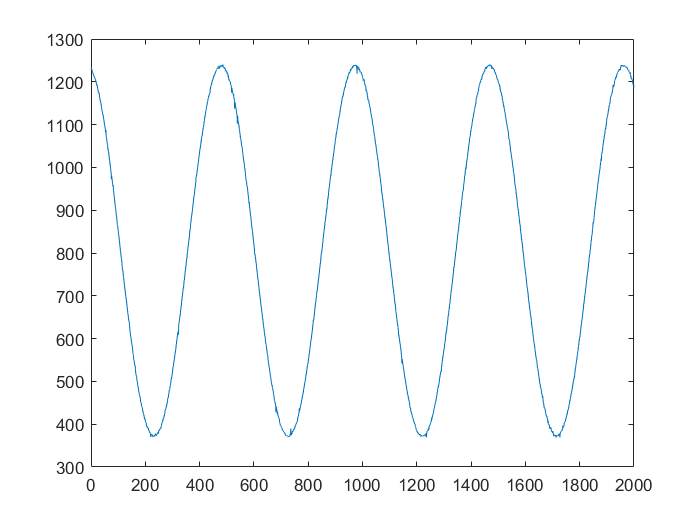
\includegraphics[width=\textwidth]{assets/exp6/onda_2kHz_8picchi.png}
\caption{Plot dei dati ricevuti}
\end{figure}